%%This is a very basic article template.
%%There is just one section and two subsections.
\documentclass[12pt]{article}
\usepackage[latin1]{inputenc}
\usepackage[T1]{fontenc}
\usepackage{graphicx}
\usepackage[italian]{babel}
\usepackage[pointlessenum]{paralist}

\title{\textbf{Documento dei requisiti}}
\date{ver. 0.1 Ultimo aggiornamento: 11-12-2008}
\author{}

\begin{document}

\maketitle

\section{Introduzione}
Il sistema software da realizzare consiste in un plugin per la piattaforma di
sviluppo Eclipse. Il plugin deve permettere l'utilizzo del tool gi�
esistente TwoTowers scritto in linguaggio C che attualmente ha una interfaccia
grafica realizzata con le librerie Tcl/Tk. Oltre alla riprogettazione e
reimplementazione della GUI preesistente, essa deve essere estesa al fine di
includere nuove funzionalit� richieste.
Nel seguito del documento verranno descritti puntualmente i requisiti funzionali
e non funzionali del progetto software.

\section{Requisiti}

\subsection{Requisiti funzionali}
\subsubsection{Obiettivi primari}

\begin{enumerate}
  
  \item L'interfaccia grafica del plugin deve permettere l'accesso a tutte le
  funzionalit� del tool TwoTowers versione 5.1 gi� presente elencate di seguito:
  \begin{enumerate}
    \item Operazioni standard su file che elabora il programma, quali:
    \begin{enumerate}
      \item visualizzazione e modifica;
      \item creazione;
      \item caricamento;
      \item salvataggio con nome;
      \item salvataggio (senza un nome nuovo);
    \end{enumerate}
    
    \item Aemilia COMPILER
    \begin{itemize}
      \item Parser
      \item Integrated semantic model size calculator
      \item Functional semantic model size calculator
      \item Performance semantic model size calculator
      \item Integrated semantic model generator
      \item Functional semantic model generator
      \item Performance semantic model generator
    \end{itemize}
    \item EQUIVALENCE VERIFIER
    \begin{itemize}
      \item Strong bisimulation equivalence verifier
      \item Weak  bisimulation equivalence verifier
      \item Strong Markovian bisimulation equivalence verifier
      \item Weak Markovian bisimulation equivalence verifier
    \end{itemize}
    \item MODEL CHECKER
    \begin{itemize}
      \item Symbolic LTL model checker
    \end{itemize}
    
    \item SECURITY ANALYZER
    \begin{itemize}
      \item Non-interference analyzer
      \item Non-deducibility on composition analyzer
    \end{itemize}
    
    \item PERFORMANCE EVALUATOR
    \begin{itemize}
      \item Stationary probability distribution calculator (Gaussian Elimination)
      \item Stationary probability distribution calculator (adaptive symmetric SOR)
      \item Transient probability distribution calculator (uniformization)
      \item Stationary reward-based measure calculator (Gaussian Elimination)
      \item	Stationary reward-based measure calculator (adaptive symmetric SOR)
      \item Transient reward-based measure calculator (uniformization)
      \item Simulator
    \end{itemize}
    
  \end{enumerate}
  
  \item Inoltre devono essere aggiunti i seguenti men� e sottomen�:
  \begin{enumerate}
    \item Architectural Assistant:
    \begin{itemize}
      \item Compatibility Checker
      \item Interoperability Checker
      \item Queueing Network Generator
    \end{itemize}
    \item Code Generator:
    \begin{itemize}
      \item Program Generator
      \item Package Generator
      \item Applet Generator
    \end{itemize}
    
  \end{enumerate}
  
  \item Integrazione dell'interfaccia realizzata con un
  tool esistente per la trasformazione di diagrammi UML in specifiche Aemilia.
  
  \item Stesura di un manuale utente, ovvero di un men� Help.
  
  \item Codice sorgente commentato e documentato attendendosi il
  pi� possibile allo stile di documentazione standard per i plugin di Eclipse.
  
\end{enumerate}

\subsubsection{Obiettivi secondari}
\begin{enumerate}
  \item Funzionalit� di editing dei file avanzate per ciascun tipo di estensione
  usato:
  \begin{itemize}
    \item syntax highlighting;
    \item content assist (per i file modificabili da utente).
  \end{itemize}
\end{enumerate}

\begin{figure}[htp]
\begin{center}
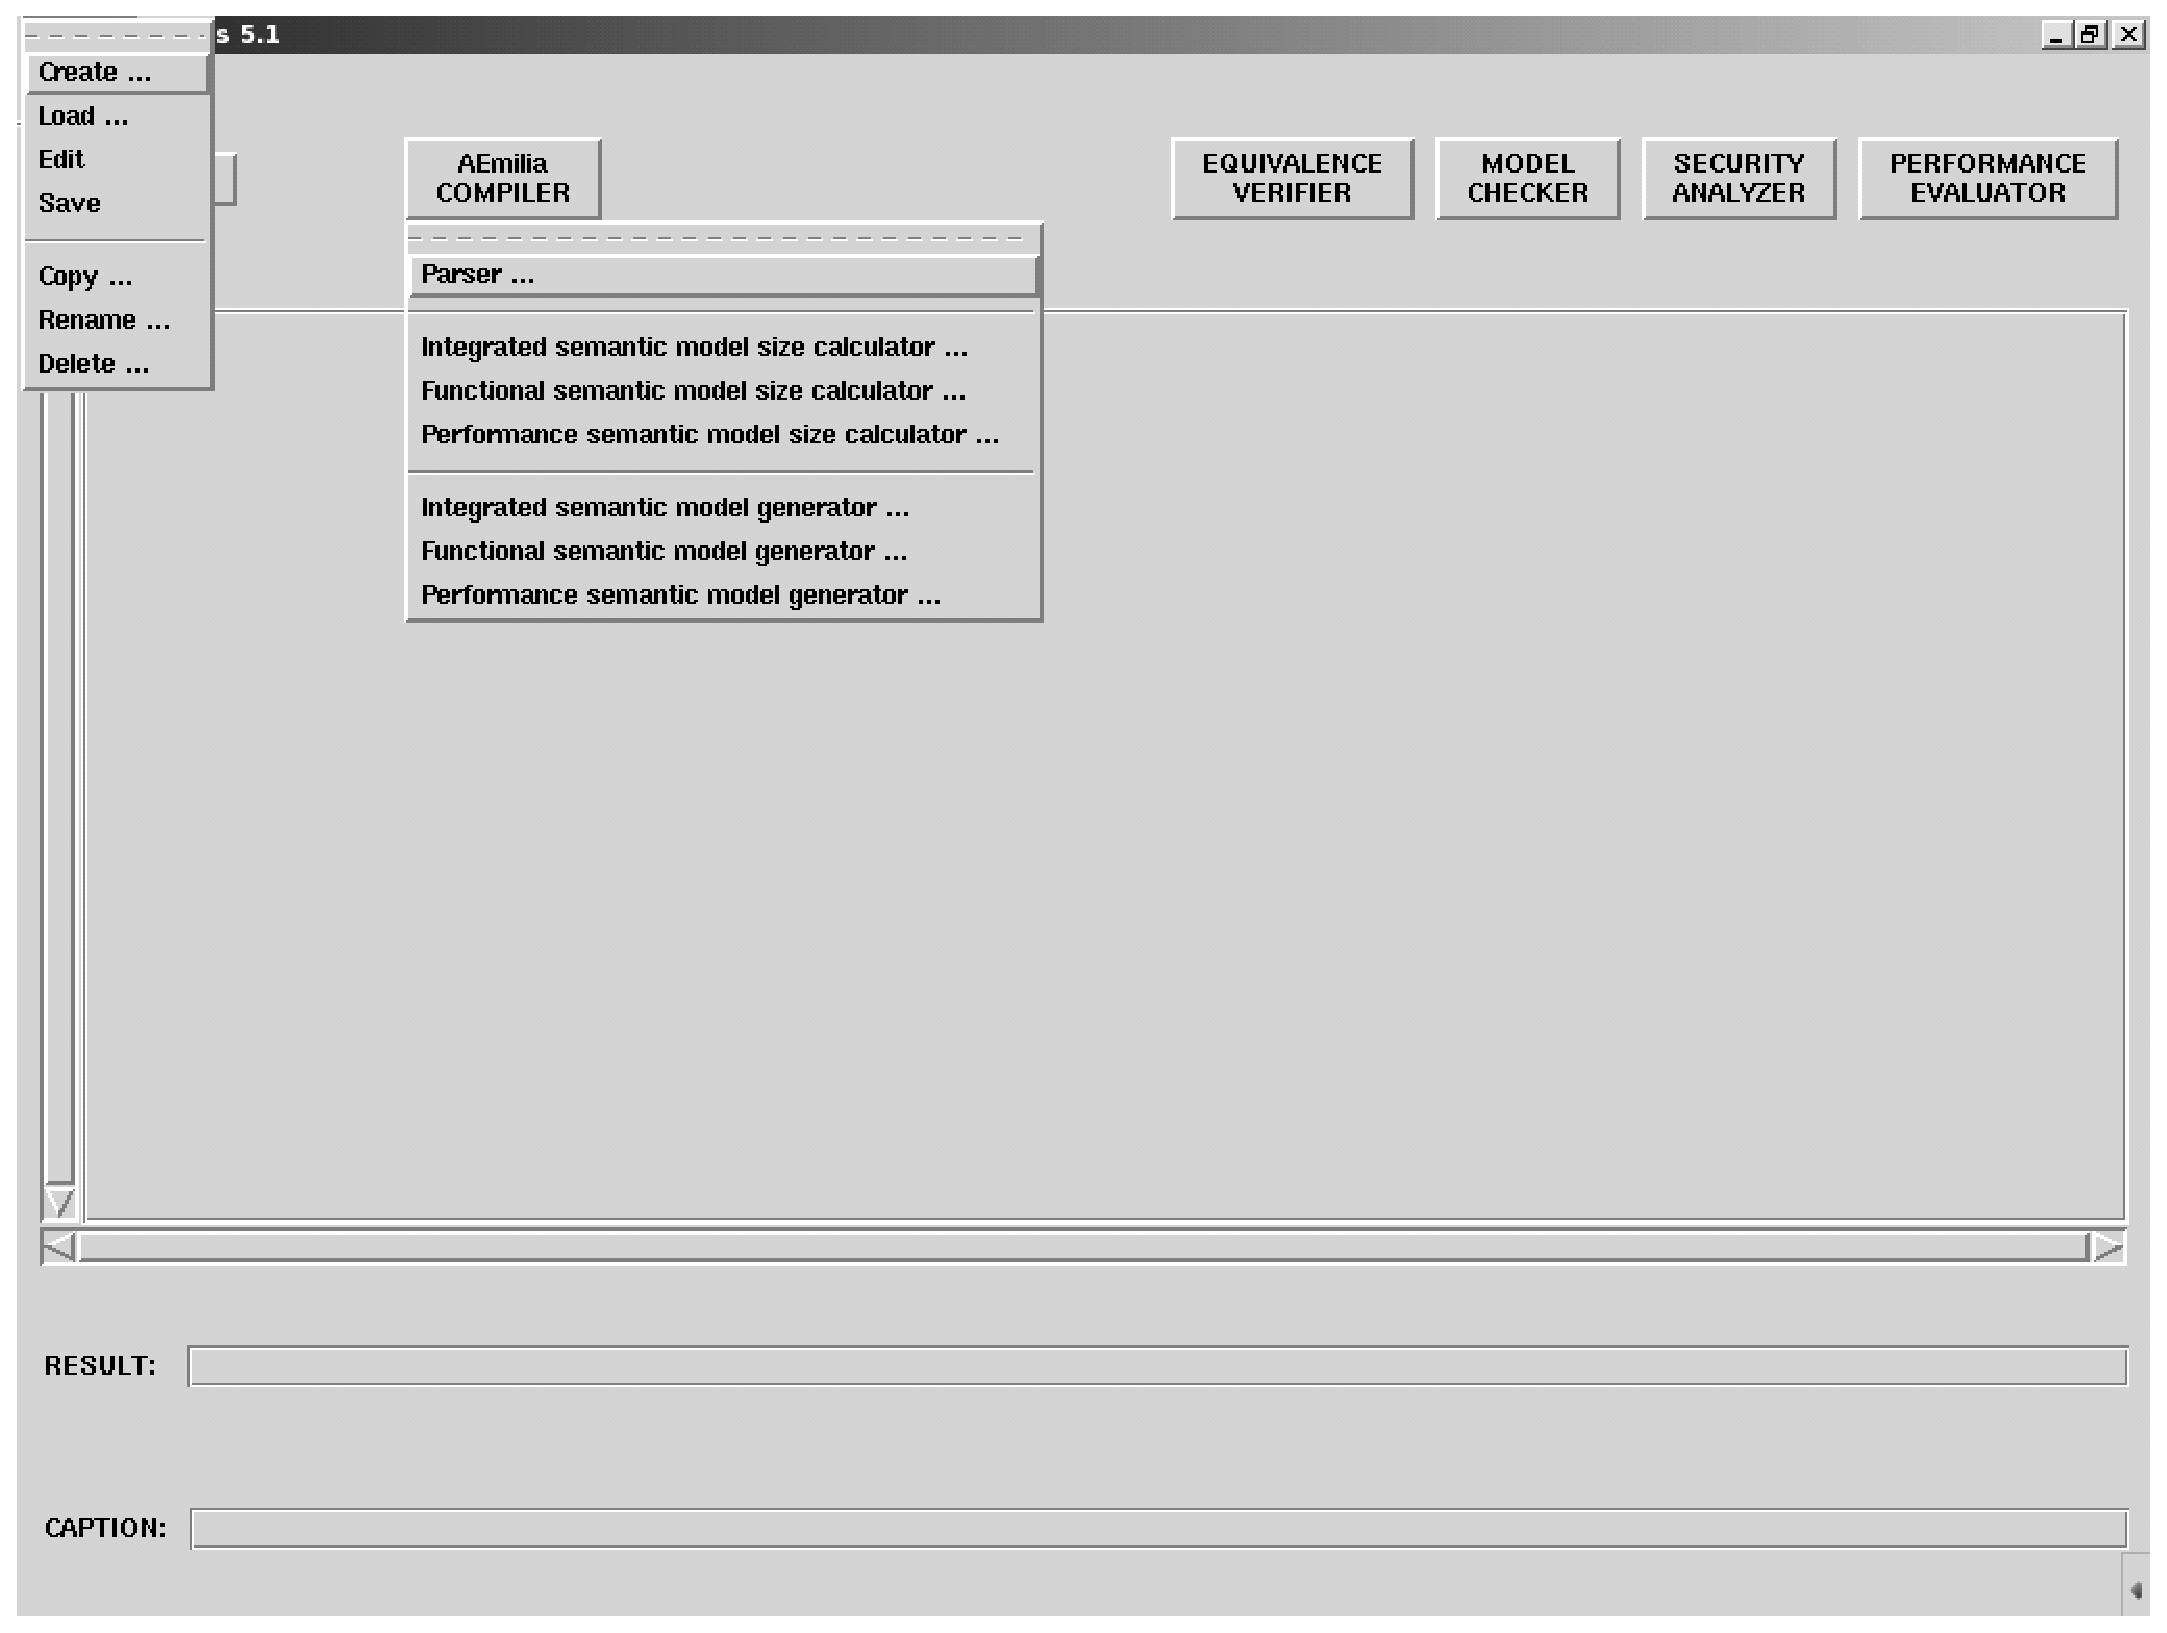
\includegraphics[width=1.2\textwidth]{compiler}
\caption[labelInTOC]{Schermata della versione 5.1 in Tcl/Tk del men�
Compiler.}
\label{compiler}
\end{center}
\end{figure}

\begin{figure}[htp]
\begin{center}
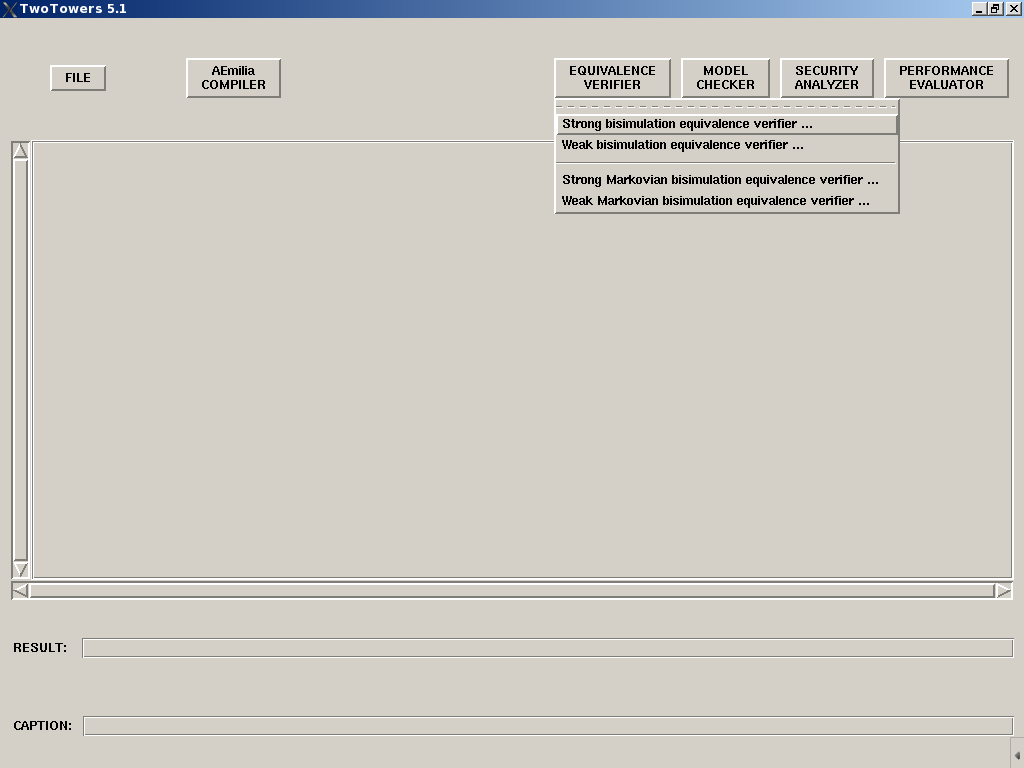
\includegraphics[width=1.2\textwidth]{equivalence}
\caption[labelInTOC]{Schermata della versione 5.1 in Tcl/Tk del men�
Equivalence Verifier.}
\label{equivalence}
\end{center}
\end{figure}

\begin{figure}[htp]
\begin{center}
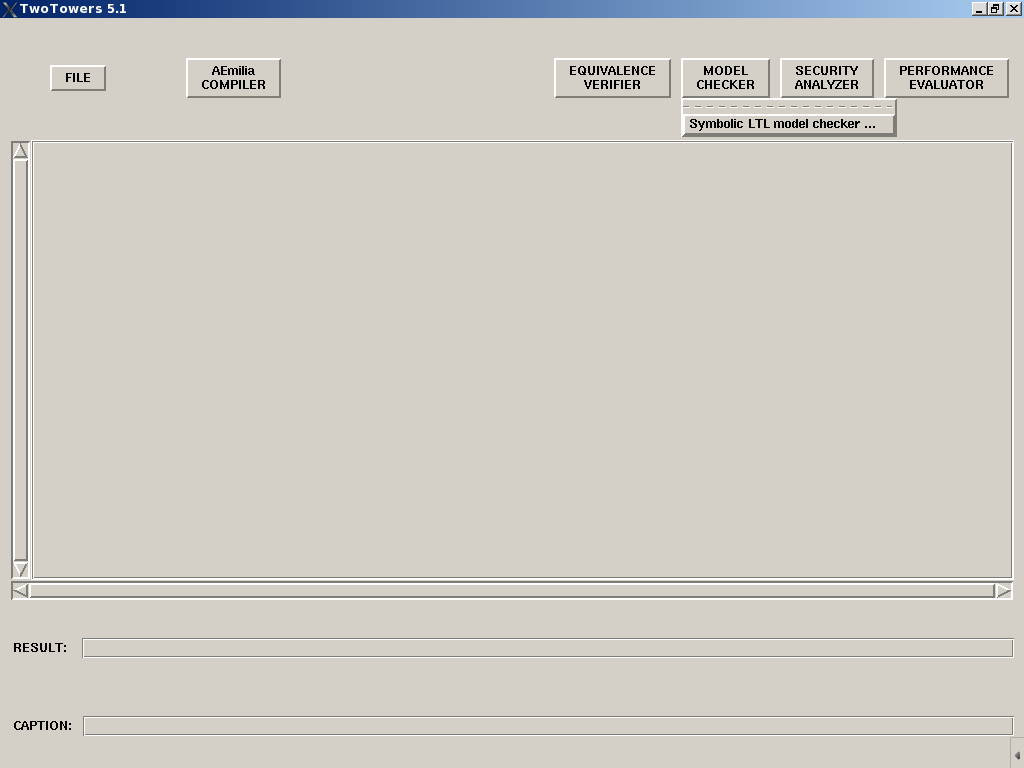
\includegraphics[width=1.2\textwidth]{model}
\caption[labelInTOC]{Schermata della versione 5.1 in Tcl/Tk del men� Model
Checker.}
\label{equivalence}
\end{center}
\end{figure}

\begin{figure}[htp]
\begin{center}
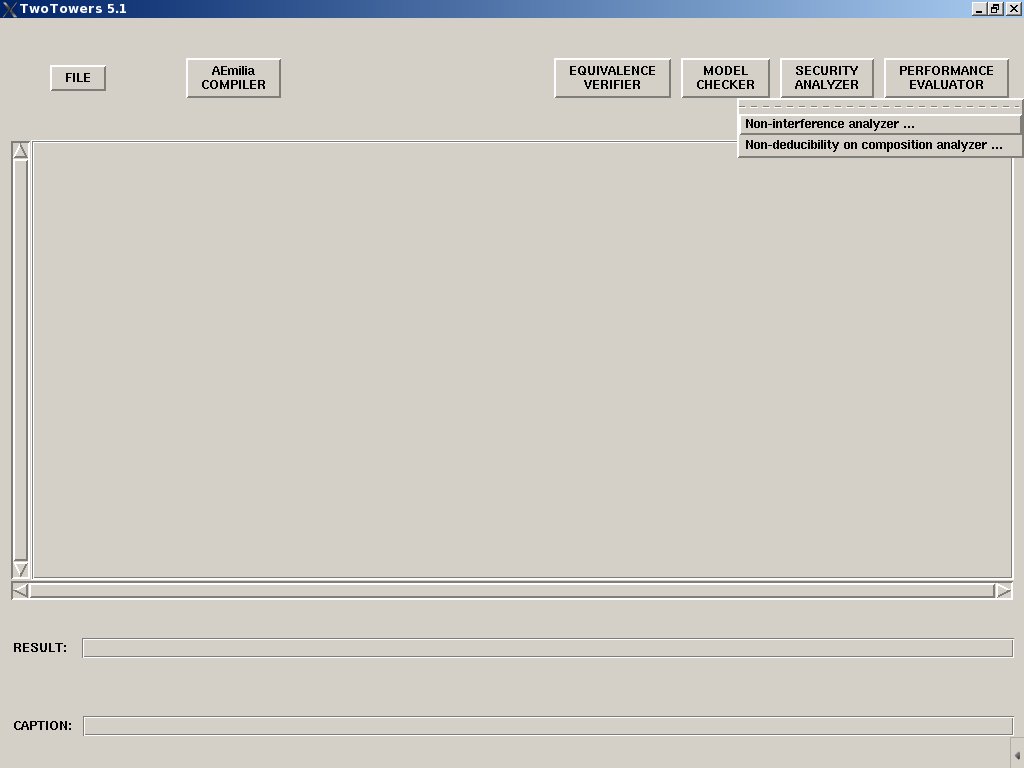
\includegraphics[width=1.2\textwidth]{security}
\caption[labelInTOC]{Schermata della versione 5.1 in Tcl/Tk del men� Security
Analyzer.}
\label{secutity}
\end{center}
\end{figure}

\begin{figure}[htp]
\begin{center}
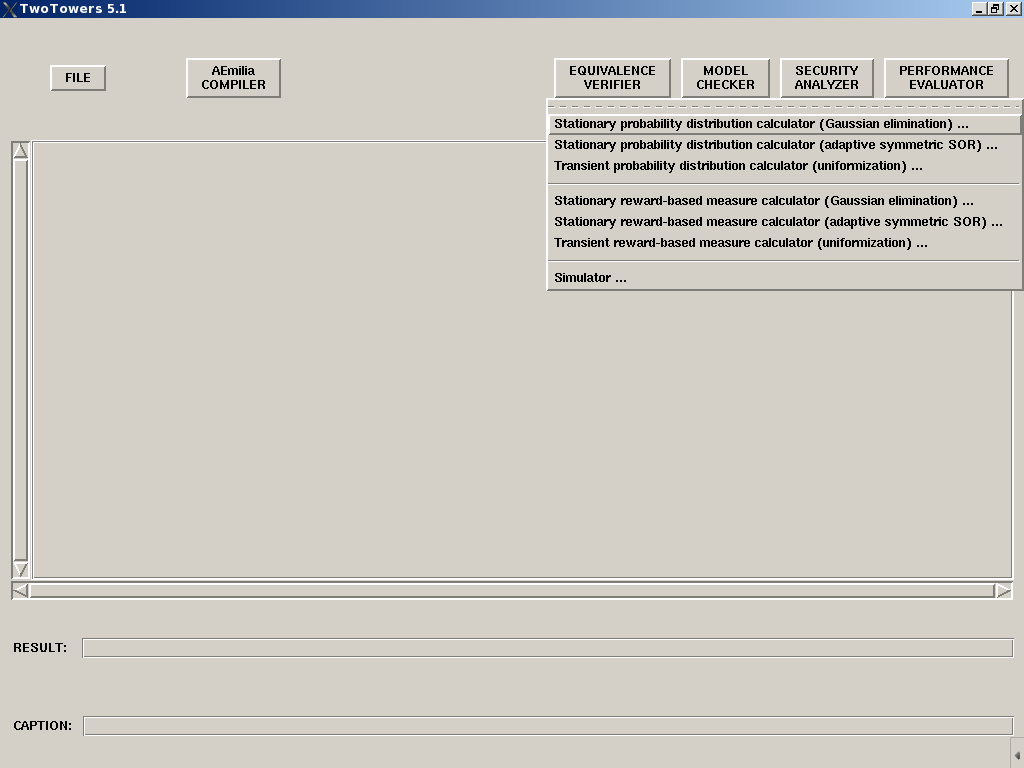
\includegraphics[width=1.2\textwidth]{performance}
\caption[labelInTOC]{Schermata della versione 5.1 in Tcl/Tk del men�
Performance Evaluator.}
\label{performance}
\end{center}
\end{figure}

\begin{figure}[htp]
\begin{center}
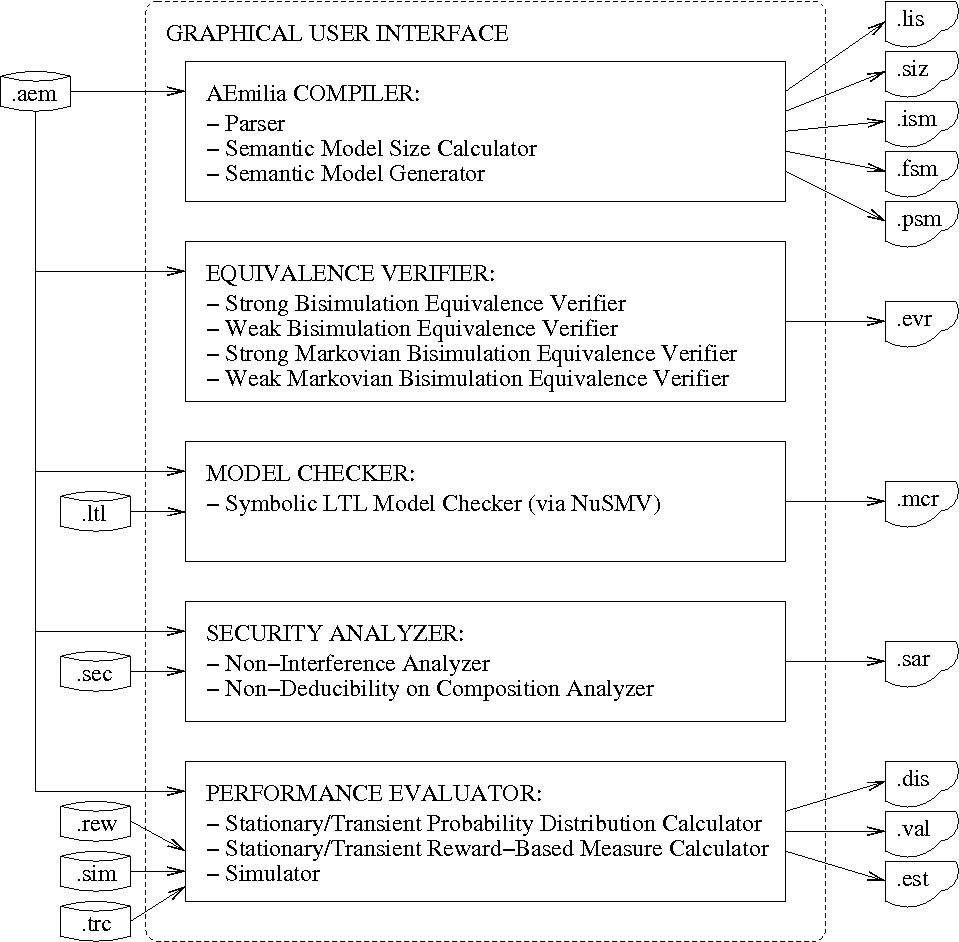
\includegraphics[width=1.2\textwidth]{twotowers}
\caption[labelInTOC]{Schermata della struttura del tool TwoTowers e delle
estensioni dei file usate.}
\label{performance}
\end{center}
\end{figure}

\subsection{Requisiti non funzionali}
Interfaccia grafica:
\begin{enumerate}
  \item intuitiva;
  \item di facile navigabilit�;
  \item estendibile.
\end{enumerate}

\subsection{Requisiti software}
Il plugin sar� sviluppato per:
\begin{itemize}
  \item Eclipse Ganymede versione 3.4.1;
  \item Java Runtime Environment versione 6.
\end{itemize}

\end{document}
